
% Basic setup. Most papers should leave these options alone.
\documentclass[a4paper,fleqn,usenatbib]{../mnras}

\usepackage{newtxtext,newtxmath}

% Use vector fonts, so it zooms properly in on-screen viewing software
% Don't change these lines unless you know what you are doing
\usepackage[T1]{fontenc}
\usepackage{ae,aecompl}


%%%%% PACKAGES %%%%%

% Only include extra packages if you really need them. Common packages are:
\usepackage{graphicx}	% Including figure files
\usepackage{amsmath}	% Advanced maths commands
\usepackage{amssymb}	% Extra maths symbols
\usepackage{color}
\usepackage{enumerate}

%%%%% CUSTOM COMMANDS %%%%%

\newcommand{\Nant}{\ensuremath{N_{\mathrm{a}}}}
\newcommand{\Ng}{\ensuremath{N_{\mathrm{g}}}}
\newcommand{\s}{\ensuremath{\hat{\mathbf{s}}}} % s-hat for sine-projected direction
\newcommand{\spix}{\ensuremath{\hat{\mathbf{s}}_{0}}}
\newcommand{\Cna}[1][n]{\ensuremath{\mathcal{C}^{(#1)}_{a,\spix}}}
\newcommand{\ri}{\ensuremath{\mathbf{r}_i}}
\newcommand{\ra}{\ensuremath{\mathbf{r}_a}}
\newcommand{\rb}{\ensuremath{\mathbf{r}_b}}
\newcommand{\beamr}{\ensuremath{\widetilde{W}}}
\newcommand{\beamtheta}{\ensuremath{W}}
\newcommand{\Er}[1]{\ensuremath{\widetilde{E}_{#1}}}
\newcommand{\Erest}[1]{\ensuremath{\widetilde{E}'_{#1}}}
\newcommand{\Ethetaest}{\ensuremath{E'}}
\newcommand{\V}{\ensuremath{\widetilde{V}}}
\newcommand{\dif}{\mathrm{d}}
\newcommand{\caliter}{400}
\newcommand{\damp}{\ensuremath{\gamma}}
\newcommand{\itr}{20}
\newcommand{\tcal}{\ensuremath{t_{\mathrm{cal}}}}
\newcommand{\teff}{\ensuremath{t_{\mathrm{eff}}}}

%%%%%%%%%%%%%%%%%%% TITLE PAGE %%%%%%%%%%%%%%%%%%%

% Title of the paper, and the short title which is used in the headers.
% Keep the title short and informative.
\title[EPICal]{An efficient feedback calibration algorithm for direct imaging radio telescopes
%The E-field Parallel Imaging Calibration Algorithm for Next-Generation Radio Telescopes
}

% The list of authors, and the short list which is used in the headers.
% If you need two or more lines of authors, add an extra line using \newauthor
\author[Beardsley et al.]{
Adam P. Beardsley,$^{1}$\thanks{E-mail: Adam.Beardsley@asu.edu}
Nithyanandan Thyagarajan,$^{1}$
Judd D. Bowman$^{1}$
\newauthor
and Miguel F. Morales$^{2}$
\\
% List of institutions
$^{1}$Arizona State University, School of Earth and Space Exploration, Tempe, AZ 85287, USA\\
$^{2}$University of Washington, Department of Physics, Seattle, WA 98195, USA\\
}

% These dates will be filled out by the publisher
\date{Accepted XXX. Received YYY; in original form ZZZ}

% Enter the current year, for the copyright statements etc.
\pubyear{2016}

% Don't change these lines
\begin{document}
\label{firstpage}
\pagerange{\pageref{firstpage}--\pageref{lastpage}}
\maketitle

% Abstract of the paper
\begin{abstract}
We present the E-field Parallel Imaging Calibration (EPICal) algorithm, which addresses the need for a real-time calibration method for direct imaging radio astronomy correlators. Direct imaging involves a spatial fast Fourier transform of antenna voltages, alleviating the harsh $\mathcal{O}(\Nant^2)$ computational scaling to a more gentle $\mathcal{O}(\Nant \log_2 \Nant)$, which can save orders of magnitude in computation cost for next generation arrays consisting of hundreds to thousands of antennas. However, because signals are mixed in the correlator, gain correction must be applied on the front end. We develop the EPICal algorithm to form gain solutions in real time without ever forming visibilities. This method scales as the number of antennas, and produces results comparable to those from visibilities. Through simulations and application to Long Wavelength Array data we show this algorithm is a promising solution for next generation instruments.
\end{abstract}

\begin{keywords}
instrumentation: interferometers -- techniques: image processing -- techniques: interferometric
\end{keywords}


%%%%%%%%%%%%%%%%% BODY OF PAPER %%%%%%%%%%%%%%%%%%

\section{Introduction}
In order to satisfy the survey speeds required for precision cosmology as well as searches for fast radio transients, radio astronomy is undergoing a paradigm shift toward interferometers consisting of hundreds to thousands of small, widefield antennas. Many arrays with this design are already built or under construction including the Hydrogen Epoch of Reionization Array\footnote{http://reionization.org} (HERA), the Murchison Widefield Array (MWA; \citealt{tin13,bow13}), the Donald C. Backer Precision Array for Probing the Epoch of Reionization (PAPER; \citealt{par10}), the LOw Frequency ARray (LOFAR; \citealt{van13}), the Canadian Hydrogen Intensity Mapping Experiment (CHIME,\citealt{ban14}), the Long Wavelength Array (LWA, \citealt{ell13}), and the low frequency Square Kilometer Array (SKA1-Low \citealt{mel13}).

Traditional radio correlators cross-multiply the voltage signals from all pairs of antennas, and the computation scales as the number of antennas squared, $\mathcal{O}(\Nant^2)$ \citep{bun04}. As the number of elements in future arrays grows, the computational cost will become prohibitively expensive, and exploring efficient correlator schemes is essential to enable next generation instruments \citep{lon00}. Meanwhile, radio transient monitoring requires access to high time and frequency resolution data to identify and characterize events such as fast radio bursts (FRBs, \citealt{lor07}), or to follow up gravitational wave candidates with radio observations \citep{abb16a,abb16b}. FRBs are highly unexplored at low frequencies (< 1 GHz), but are expected to occur on timescales $\Delta t \sim$ 1--10~ms \citep{tho13}. Recording the full visibility matrix for $\Nant \gtrsim 10^3$ arrays at this timescale leads to extremely high data write rates. 

Direct imaging correlators are a new variety of radio correlator which aim to alleviate both the computational strain of forming $\Nant^2$ correlations and the high data throughput associated with short timescale science. This is done by performing a spatial fast Fourier transform (FFT) to image the antenna voltages, then squaring and averaging in time. This process scales as $\mathcal{O}(\Ng \log_2 \Ng)$, where \Ng~is the number of grid points in the FFT \citep{mor11, teg09, teg10}. For certain classes of telescopes, significantly those envisioned for next generation cosmology experiments, this scaling is a large improvement over the $\Nant^2$ scaling of traditional methods. Furthermore, because images are generated online, the native output bandwidth will be lowered (assuming $\Ng < \Nant^2$), and has the potential to be lowered even further with online transient processing.

A handful of prototype direct imaging correlators have been tested on arrays including the Basic Element for SKA Training II (BEST-2) array \citep{fos14}, the Omniscope \citep{zhe14}, and an earlier pulsar timing experiment at GHz frequencies \citep{oto94, dai00}. Each of these are examples of so-called FFT correlators -- a subclass of direct imaging correlators which rely on identical antennas with restricted placement, which allows the FFT to be performed without gridding. We recently released the E-field Parallel Imaging Correlator \citep[EPIC;][]{thy15c}, which is a software implementation of the Modular Optimal Frequency Fourier \citep[MOFF;][]{mor11} imaging algorithm. This architecture leverages the software holography/A-transpose framework to grid electric field data streams before performing the spatial FFT, allowing for an optimal map without placing constraints on array layout or requiring identical antennas \citep{mor09,bha08,teg97a}.

A challenge common to all direct imaging algorithms is calibration of the antenna gains. With a traditional FX or XF correlator, pair-wise visibilities are written to disk and used to calibrate offline before further processing such as imaging. However, a direct imaging correlator mixes the signals from all antennas before averaging and writing to disk, making calibration a requirement at the front end, before imaging and averaging. Previous solutions have involved applying calibration solutions generated from a parallel FX correlator \citep{zhe14, fos14}, or integrating a dedicated FX correlator which periodically formed the full visibility matrix to solve for gains \citep{wij09,dev09}. While these solutions were sufficient to enable the exploration of FFT correlators and beamformers, they will not scale to future arrays with $\Nant \gtrsim 10^3$.

Here we present the E-field Parallel Imaging Calibration (EPICal) algorithm -- a novel solution to the calibration problem, which can be integrated into direct imaging correlators and scales only as the number of antennas, $\mathcal{O}(\Nant)$. This method uses a correlation of the uncalibrated antenna signal stream with an output image pixel from the backend of the correlator to solve for the complex gains of the antennas. Because the calibration must be applied before gridding and imaging, our solution requires an iterative approach where the data from one time series is used to update the gains which are applied to the following time series. An example implementation of the algorithm is available with the EPIC software package\footnote{http://github.com/nithyanandan/EPIC}.

We review the MOFF algorithm and derive the calibration algorithm in \S \ref{sec:math}. We then demonstrate the algorithm in simulations in \S \ref{sec:sim}, and apply to a sample LWA data set in \S \ref{sec:data}. Then we discuss errors and noise properties of the resulting gain solutions in \S \ref{sec:noise}. Finally we conclude and discuss potential extensions to the algorithm in \S \ref{sec:discussion}.

\section{Mathematical Framework}\label{sec:math}
\subsection{Review of the MOFF algorithm}
We begin by reviewing the data flow of the MOFF algorithm, highlighting aspects relevant to the calibration. The interested reader is encouraged to refer to \citealt{mor11} for a more thorough discussion. Figure~\ref{fig:moff_flow} is reproduced from \citealt{thy15c} to illustrate the various steps of the algorithm.

\begin{figure}
\begin{center}
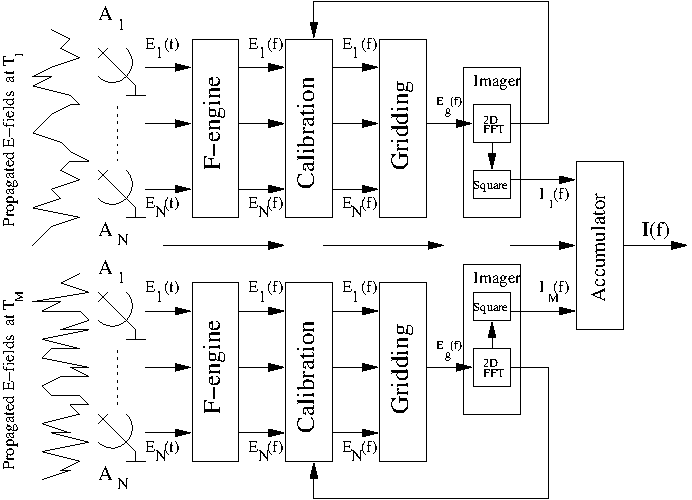
\includegraphics[width=\columnwidth]{figures/MOFF_flowchart.pdf}
\caption{Data flow for the MOFF algorithm, reproduced from \citealt{thy15c}. The time ordered electric fields are collected by the antenna elements then frequency transformed in the F-engine. The calibration is applied, then the electric field measurements are gridded using the antenna voltage patterns. The imager performs a spatial 2D FFT on the gridded data before squaring and averaging. The accumulated images are then written to disk.}
\label{fig:moff_flow}
\end{center}
\end{figure}

The electric field incident on the ground, $\Er{}(\mathbf{r},t)$, is related to the sky electric field, $E(\hat{\mathbf{s}},t)$, through a Fourier transform.
\begin{equation}
\Er{}(\mathbf{r},t) = \int E(\hat{\mathbf{s}},t) e^{-2\pi i \mathbf{r}\cdot \hat{\mathbf{s}}}\, \dif^2 \hat{\mathbf{s}}
\end{equation}
Here $\hat{\mathbf{s}}$ denotes the sine-projected unit vector for the sky angle, $\mathbf{r}$ is the observer's location (measured in wavelengths relative to an arbitrary origin). We will encounter several quantities which we attempt to estimate. We distinguish the ``true'' values with a superscript $T$, while the estimated quantities are denoted with a prime. We define the true antenna signal as a convolution of the antenna voltage pattern, \beamr, with the electric field on the ground.
\begin{equation}
\Er{a}^T(t) \equiv \int \beamr_a(\mathbf{r}-\ra) \Er{}(\mathbf{r},t) \, \dif^2 \mathbf{r}
\end{equation}
The subscript $a$ labels the antenna, and $\mathbf{r}_a$ is the location of antenna $a$. 

The first step of the MOFF algorithm is identical to the F-engine of a traditional FX correlator where the electric fields are Fourier transformed to frequency channels, $\Er{a}^T(f,t)$. Even after transforming along the time axis, we retain the time dependence of the signal to represent a stream of spectra.

Thus far we have assumed the antennas deliver the true electric field signals. Here we introduce a multiplicative complex gain as well as an additive noise term which corrupt the measured signals.
\begin{equation}\label{eq:apply_gain}
\Er{a}(f,t) = g^T_a(f,t) \Er{a}^T(f,t) + \widetilde{n}_a(f,t)
\end{equation}
Note that this quantity is neither a true or estimated value, but rather the raw electric field signal corrupted by the complex gain before we attempt to estimate the true value. The noise term is strictly receiver noise -- noise introduced by the instrument. Any sky noise is implicitly included in the time dependence of the sky electric field. We will neglect $\widetilde{n}_a$ for now, but will inspect its effects at the end of this section. Each subsequent step treats each frequency channel independently, so we will drop the $f$ to simplify notation. 

The MOFF algorithm next calls for a calibration. The goal of our new calibration method will be to form an estimate of the gains, $g'_a$. For now we will assume we have formed an estimate to proceed with the MOFF pipeline. We correct the incoming electric field data stream using our current estimate of the gains.
\begin{equation}
\Erest{a}(t) = \Er{a}(t)/ g'_a
\end{equation}

The next step is to grid the antenna signals. MOFF uses the antenna patterns as the gridding kernel according to the software holography/A-transpose technique \citep{mor09,bha08}. This achieves both an optimal map \citep{teg97b} and places the data on a regular grid. Unlike traditional correlators which grid visibilities, the MOFF grids the electric fields directly. This operation must be performed for every time step, before any averaging of the data.

After gridding, the imaging portion of the MOFF performs a 2D spatial FFT to form instantaneous electric field images of the sky. The pipeline up to this point can be summarized through the following equation.
\begin{equation}
\Ethetaest (\s_i,t) = \underbrace{\frac{1}{\Nant} \sum_i e^{2\pi i \ri \cdot \s_i}}_{\mathrm{2D\;FFT}} 
\underbrace{\sum_a \beamr_a(\ri - \ra)}_{\mathrm{Gridding}}
\underbrace{ \frac{g^T_a}{g'_a} \Er{a}^T(t)}_{\mathrm{Calibration}}
\end{equation}
The sum over antennas uses the voltage pattern to grid the calibrated electric fields onto regular gridpoint, $i$. The sum over $i$ denotes the 2D FFT to sky coordinates, resulting in an estimate for the instantaneous electric field image. We can simplify this expression by exchanging the sums to transform the beam term into sky coordinates.
\begin{align}\label{eq:epix}
\Ethetaest(\s_i,t) & = \frac{1}{\Nant} \sum_a \frac{g^T_a}{g'_a}\Er{a}^T(t) e^{2\pi i \s_i \cdot \ra} \nonumber \\
  & \qquad\times \sum_i \beamr_b(\ri-\ra)e^{2\pi i \s_i \cdot (\ri-\ra)} \nonumber\\
& = \frac{1}{\Nant} \sum_a \frac{ g^T_a}{g'_a}\Er{a}^T(t) e^{2\pi i \s_i \cdot \ra}\beamtheta_a(\s_i)
\end{align}
In this form we see that the effect of gridding with the antenna voltage pattern is to attenuate the image by a factor of the antenna sky response, $\beamtheta_a(\s_i)$.

Finally, the images are squared and averaged in time to reduce output bandwidth, then written to disk. While operations have been reordered, the resulting image is equivalent to one produced by gridding and imaging visibilities. By shifting from cross-correlation of all pairs of antennas to a spatial FFT, the computational cost is significantly lowered for certain classes of compact arrays. The output bandwidth is also greatly reduced as visibilities are exchanged for gridded images. A full exploration of these scalings was presented in \citealt{thy15c}.

\subsection{Derivation of calibration}
We saw above that the MOFF algorithm (in general any direct imaging architecture) mixes the signal from all antennas coherently, and thus requires the calibration to be applied in real time at the front end of the correlator. Furthermore, visibilities are never formed, which are traditionally the basic measurement used to form calibration solutions. Here we derive an alternative method to estimate the antenna gains in real time, using the data products of the MOFF. 

Because the gains must be estimated in real time, we will need to use a finite stream of data to form and estimate which will be applied to the subsequent stream of data. Therefore the process of finding a solution is an iterative one. We will use parenthetical superscripts to denote the calibration loop number. For example, we will assume we have already formed an estimate from $n$ loops, $g^{(n)}_a$. We will use these estimates to calibrate the next stream of data in order to form an updated estimate, $g^{(n+1)}_a$.

As a starting point, we consider the feedback calibration outlined in \citealt{mor11}. There it was suggested to form a correlation of the uncalibrated antenna measurements with an image pixel from the output of the correlator. This is a statistically stationary quantity, which can be related to the sum of visibilities involving the antenna used in the correlation -- exactly the sum needed to calibrate a simple sky of a single point source. However, we aim for a more generalized solution for arbitrarily complex sky models. We therefore study the full expression for the antenna-pixel correlation,
\begin{equation}\label{eq:Cna}
\Cna \equiv \left<\Er{a}(t) E'^*(\spix,t)\right>_t,
\end{equation}
where the superscript $n$ again represents the quantity formed in the $n^\mathrm{th}$ calibration loop, and \spix\, is the pixel center nearest a bright calibrator of interest. The following will hold for any chosen pixel, \spix, though it is advantageous to choose a pixel which contains a bright source to achieve a high signal to noise. 

Plugging equation \ref{eq:epix} into equation \ref{eq:Cna}, we find,
\begin{align}\label{eq:cna}
\Cna & = \left<g^T_a \Er{a}^T(t) \frac{1}{\Nant} \sum_b \frac{g^{T*}_b}{g^{*(n)}_b}\Er{b}^{T*}(t) e^{-2\pi i \spix \cdot \rb} \beamtheta^*_b(\spix)\right>_t \nonumber \\
& = \frac{g^T_a}{\Nant} \sum_b \frac{g^{T*}_b}{g^{*(n)}_b} \beamtheta^*_b(\spix) e^{-2\pi i \spix \cdot \rb} \left<\Er{a}^T \Er{b}^{*T} \right>_t \nonumber \\
& = \frac{g^T_a}{\Nant} \sum_b \frac{g^{T*}_b}{g^{*(n)}_b} \beamtheta^*_b(\spix) e^{-2\pi i \spix \cdot \rb} \V^T_{ab}
\end{align}
where in the second step we group time-dependent terms, and in the third we define the true visibilities as the correlation between true antenna electric field measurements. It is easy to see from here that the net effect of including the receiver noise term, $\widetilde{n}_a(f,t)$, will result in added noise on the true visibilities, including a bias on the auto-correlation terms. In principle a bias can result on any visibility from any noise correlations between antennas, but the implementation included in the EPIC software package restricts the noise term to include only the auto-correlation noise bias, and assumes baseline dependent noise has zero mean.

The next step is to use this antenna-pixel correlation to update our gain solution. We will model the right hand side of equation~\ref{eq:cna} by assuming our current gain estimates are approximately correct, $g^{(n)}_b\approx g^T_b$, and replacing the true visibilities with a set of model visibilities, $\V'_{ab}$. These model visibilities rely an knowledge of the sky, and should be precomputed offline. We can then solve equation~\ref{eq:cna} for $g^T_a$ to achieve an updated estimate.
\begin{equation}\label{eq:cal_solution}
g'^{(n+1)}_a = \Cna \Nant \left[ \sum_b \beamtheta^*_b(\spix) e^{-2\pi i \spix \cdot \rb} \V'_{ab} \right]^{-1}
\end{equation}
This equation is our prescription for estimating the antenna gains of a direct imaging array. The online computation complexity scales as $\mathcal{O}(\Nant)$ as we form a $\Cna$ for each antenna. 

We show schematically the process of calibrating a direct imaging correlator in figure~\ref{fig:schematic}. Computationally expensive steps that must be performed ``on-chip" are shown inside the gray box. The uncalibrated antenna signals are tapped out after the F-engine and correlated against the output image pixel of interest (i.e., equation~\ref{eq:Cna} is ``on-chip''). The correlated values are then passed off-chip to estimate the gains using equation~\ref{eq:cal_solution}, and additional fitting if desired. The gains are then passed back to the correlator to update the calibration for subsequent integration intervals. 

\begin{figure}
\begin{center}
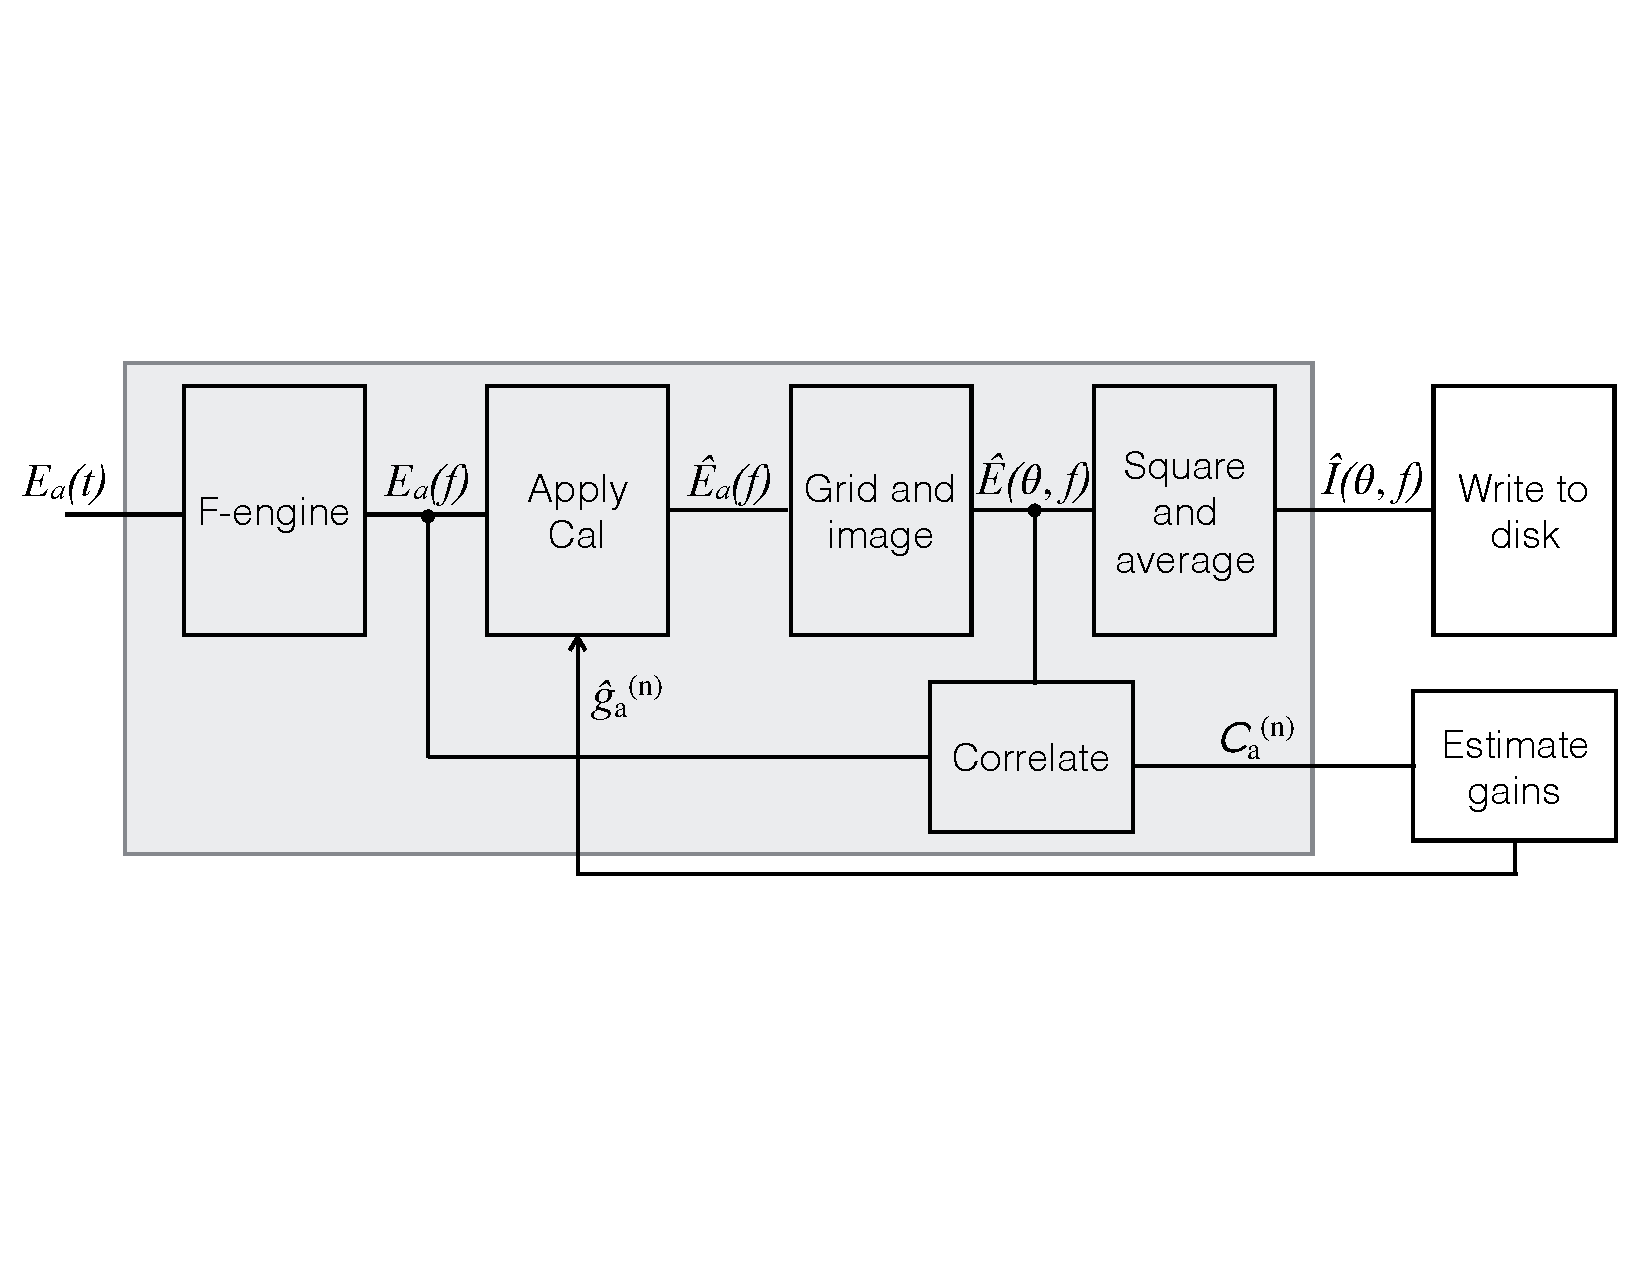
\includegraphics[width=\columnwidth]{figures/schematic.pdf}
\caption{The general data flow of the MOFF correlator, with a feedback calibration loop. A pixel from the (unsquared) image is tapped out and correlated against the input antenna electric field signals to form $\Cna$ coefficients (equation~\ref{eq:Cna}). These coefficients are then shipped off-chip to apply equations~\ref{eq:cal_solution}~and~\ref{eq:damping}, and any other processing to arrive at an updated estimate of the gains, $g^{(n)}_a$. The gray box shows operations which must be done at high speed (before averaging in time), which white boxes show operations which can be performed ``off-chip".}
\label{fig:schematic}
\end{center}
\end{figure}

While testing we found equation~\ref{eq:cal_solution} resulted in oscillatory gain solutions as it was iterated, as is often the case in iterative minimization methods. To mitigate this we introduce a damping factor, $0 \leq \damp <1$, which is used to attenuate the gain update, effectively giving the solutions memory of previous iterations.
\begin{equation}\label{eq:damping}
g^{(n+1)}_a = (1-\damp) g'^{(n+1)}_a + \damp g^{(n)}_a
\end{equation}
We found that while equation~\ref{eq:cal_solution} does indeed converge on good solutions, the process is made faster by tuning the damping factor. While $g'^{(n+1)}_a$ is the best estimate of the gains after the $n^{\textrm{th}}$ iteration, the damped version, $g^{(n+1)}_a$, is actually used in the iterative calibration loop. Once the loop converges the damped version is essentially a weighted average over the past several iterations, giving it a longer effective integration time. 

An important feature to note is that, like the MOFF-generated images themselves, equation~\ref{eq:cal_solution} includes the antenna auto-correlations (the sum is over \emph{all} $b$, not excluding $a$). It can be difficult to perfectly model the noise bias from auto-correlations, which can often times be far brighter than the visibilities themselves. It can therefore be beneficial to subtract this term directly from \Cna, and exclude the $b=a$ term in the sum.
\begin{equation}
\Cna \rightarrow \Cna - \frac{1}{\Nant\, g^{*(n)}_a} \beamtheta^*_a(\spix) e^{-2\pi i \spix \cdot \ra} \left<|\Er{a}|^2\right>_t
\end{equation}
We have absorbed $g_a^T$ into the electric field so that the correlation is now simply the autocorrelation of the uncalibrated antenna measurement. This requires generating these correlations, which again only scale as $\mathcal{O}(\Nant)$, and are generally useful for array diagnostics.

We conclude this section by connecting our calibration expression to that found in a visibility framework. In the limit of a single bright calibrating source at phase center, we can greatly simplify equations~\ref{eq:cna} and~\ref{eq:cal_solution}. We will assume the beams are normalized such that $\beamtheta(0)=1$. We can further drop the exponential phase terms because $\spix=0$. We then absorb the true gains into the true visibilities in equation~\ref{eq:cna} to express as a sum of measured, uncalibrated, visibilities.
\begin{equation}
\mathcal{C}^{(n)}_{a,0} \rightarrow \frac{1}{\Nant}\sum_b \frac{1}{g^{*(n)}_b} \V_{ab}
\end{equation}

We next plug this expression into equation~\ref{eq:cal_solution} to find our simplified calibration solution for a single bright point source. Because our sky is a single bright point source, the model visibilities are simply the flux of the source, $S_{\mathrm{src}}$.
\begin{equation}
g'^{(n+1)}_a \rightarrow \frac{\sum_b  \V_{ab}/g^{*(n)}_b}{\Nant S_{\mathrm{src}}}
\end{equation}
This is simply a gain-weighted sum of the measured visibilities over the flux of the source, which is indeed the limiting result from a visibility approach, for example seen in \citealt{mit08}. The ability to recover the equivalent expression despite not actually forming the visibilities is a result of the fact that only sums over visibilities come into the FX solution, as was described in \citealt{mor11}. We have confirmed the limiting case equivalence here, and will explore the more general case in more detail in \S~\ref{sec:noise}.

\section{Simulation}\label{sec:sim}
We first demonstrate our calibration method through a controlled simulation. A complex gain is created for each antenna with random phase and amplitude, which is used to corrupt the simulated data stream, then we attempt to recover the gains using our calibration routine. The simulation software used is included in the EPIC package.

Our simulated signal consists of 10 random point sources with flux densities 0.5~Jy~$\lesssim S \lesssim 1$~Jy. For an antenna array we use the inner 51 antennas of the MWA layout \citep{bea12}, within a bounding box of 150~m. The antenna voltage pattern used is a 4.4~m square tophat on the ground. Because our algorithm treats frequency channels independently, we simulate only one channel. For context we treat this channel as a single 40 kHz, meaning each subsequent timestep is separated by 25~$\mu$s.

For our unknown gains, we create a set of random complex numbers where the amplitude is drawn from approximately gaussian distribution centered around 1 with width 0.25, and completely random phase. These are our ``true gains", and we apply them to the frequency-domain simulated antenna electric fields as in equation~\ref{eq:apply_gain}. Our analysis is blind to these values until the end of the process to check accuracy. The gain estimates are initialized with unity, $g^{(0)}_a=1$.

We next process and image \caliter~time steps (10~ms). We also form the correlations, \Cna[0], used in our calibration loop. The pixel used for the correlation is the source with the largest apparent flux (intrinsic flux attenuated by the primary beam). These correlation values are used to update the gain estimates, which in turn are used to calibrate the following \caliter~time steps. Through experimentation we found a damping factor of $\damp=0.35$ resulted in the quickest convergence in this simulation.

The calibration loop continues by updating the gain estimates every \caliter~time steps. The phases of our gain estimates are shown in figure~\ref{fig:sim_phase} for 20 such iterations. The phase error plotted is the phase relative to the true gain for each antenna (various colored lines). One antenna was used as a reference to fix the absolute phase, so has zero phase error. The other 50 antennas are shown to have error spanning $2\pi$ initially, and after about 10 iterations lock into a solution, settling down to noise levels around iteration 15 (0.15~s). We stop the simulation when the updated gains trace the thermal noise of the simulated sources, which can be seen by the coherence of the 50 antenna gains after iteration 15.

\begin{figure}
\begin{center}
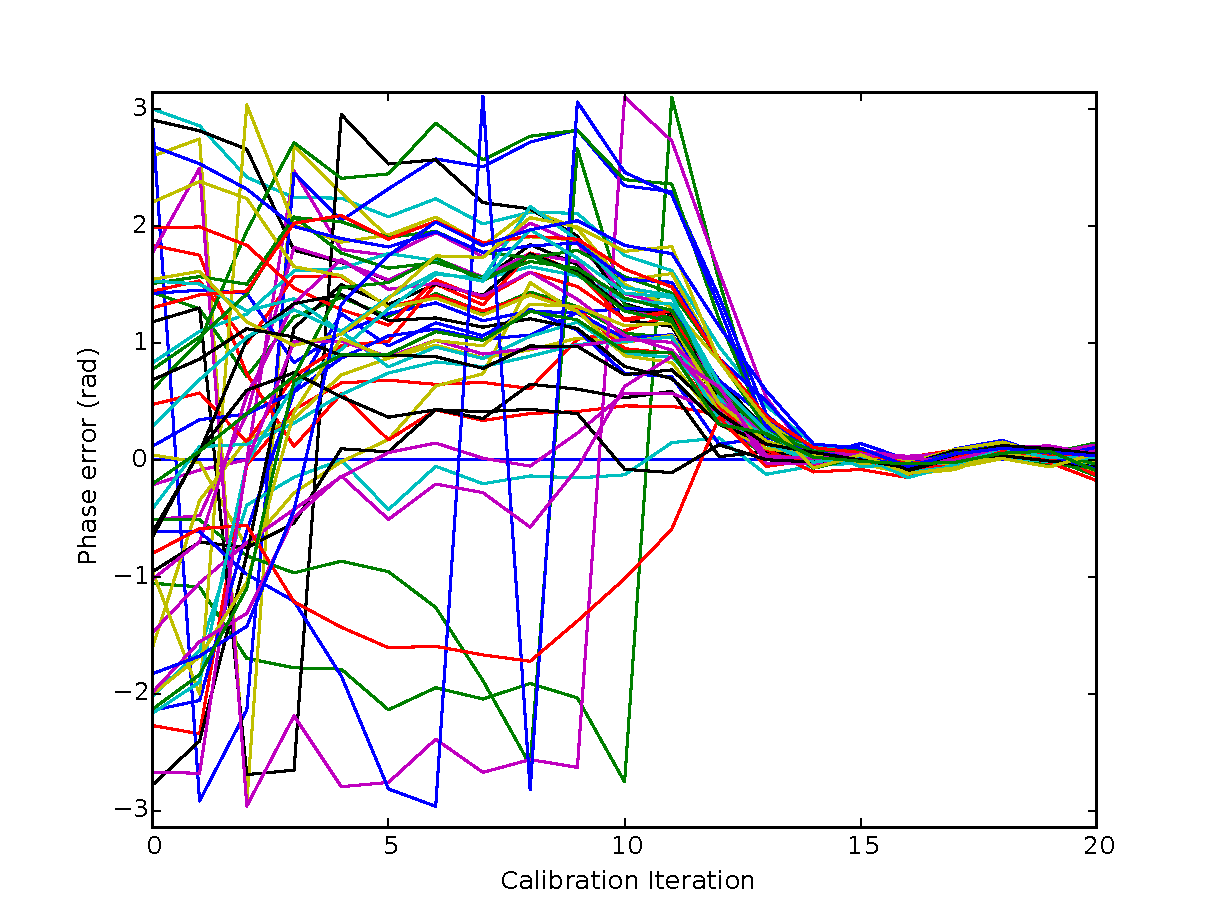
\includegraphics[width=\columnwidth]{figures/cal_paper_sim_phase.pdf}
\caption{Phase error of gain estimates as a function of iteration for simulated calibration. The gains were initialized with random phases, but the calibration loop was able to recover the correct phases after about 15 iterations. Each line represents an antenna in our 51 MWA antenna sample.
}
\label{fig:sim_phase}
\end{center}
\end{figure}

The estimated gain amplitudes for the simulations are shown in figure~\ref{fig:sim_amp}. The quantity plotted is the magnitude of the estimated gains over the true gains, $\left|g^{(n)}_a/g^T_a\right|$, which places all antennas on the same scale. We can see the amplitudes converge toward their true values around the same time as the phases (iteration $\sim$15). At the beginning of calibration we can see the value of the damping factor. At $n=0$, a couple of gains are shown to have abnormally high amplitude estimates, notably one about 3.3 times its true value (red line). These unbalanced high estimates caused the entire set of gains to be under estimated at $n=1$, even with a damping factor of 0.35. By $n=5$ the unbalanced amplitudes have been damped out and the calibration continues. Without the damping factor, the oscillation seen in the first couple iterations would have been significantly larger and taken much longer to fade out. 

\begin{figure}
\begin{center}
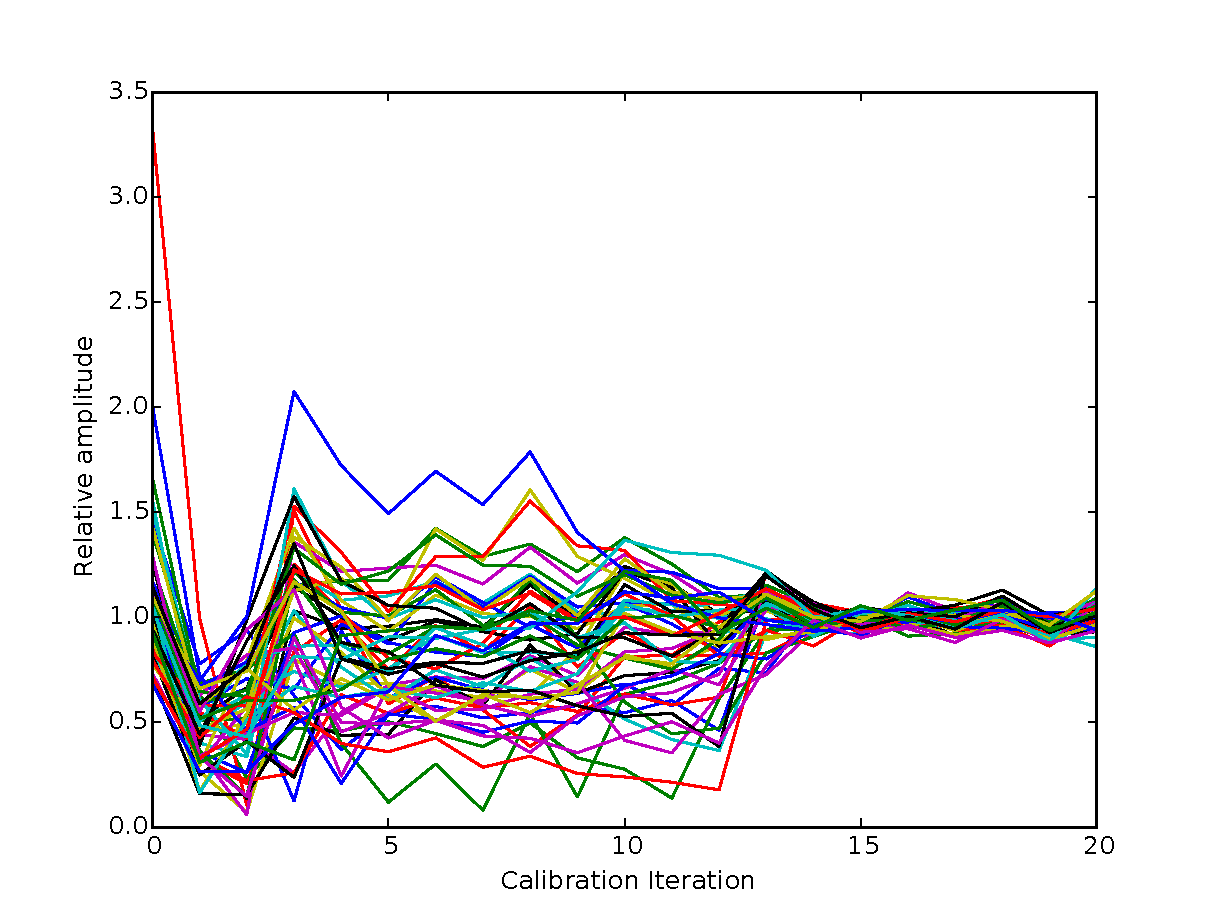
\includegraphics[width=\columnwidth]{figures/cal_paper_sim_amps.pdf}
\caption{Gain estimate amplitudes as a function of iteration for simulated calibration. Again, each line represents an antenna in the 51 MWA antenna sample. The gain estimates were initialized randomly, while the true values were unity. After about 15 iterations we see the calibration loop has settled around the correct values, with only noise remaining.}
\label{fig:sim_amp}
\end{center}
\end{figure}

After the gains have converged, we see both the phases and amplitudes to continue to fluctuate coherently. This is due to the stochastic fluctuations of the simulated sources themselves, and is limited by the sky noise. For this simulation we restricted each calibration iteration to only 10~ms integration time. In principle a calibration implementation could use short integration times to allow the gains to converge, then increase the integration time to reduce this noise.

Images created at the beginning of calibration and at the end are shown in figure~\ref{fig:sim_images}. Each image is obtained over 10~ms integration, corresponding to all snapshot images created with a given set of gain estimates. The top panel shows the image produced with our initialized unity gains. Because the phases are completely random, the image is essentially noise with the primary beam evident. After 20 iterations, the image is far more clear, shown in the bottom panel. Each of the ten simulated sources are clearly visible, indicated with red circles. 

\begin{figure}
\begin{center}
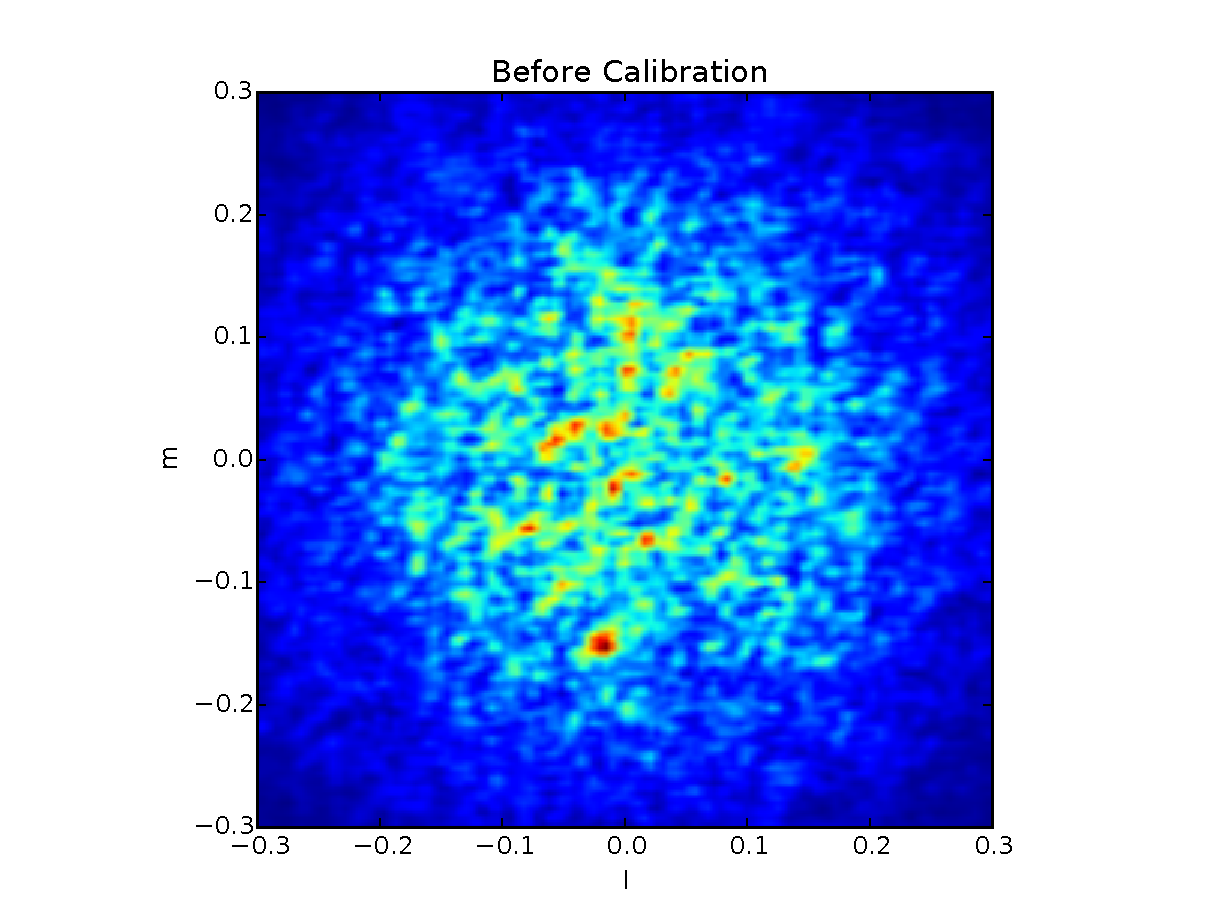
\includegraphics[width=\columnwidth]{figures/cal_paper_sim_image_before.pdf}
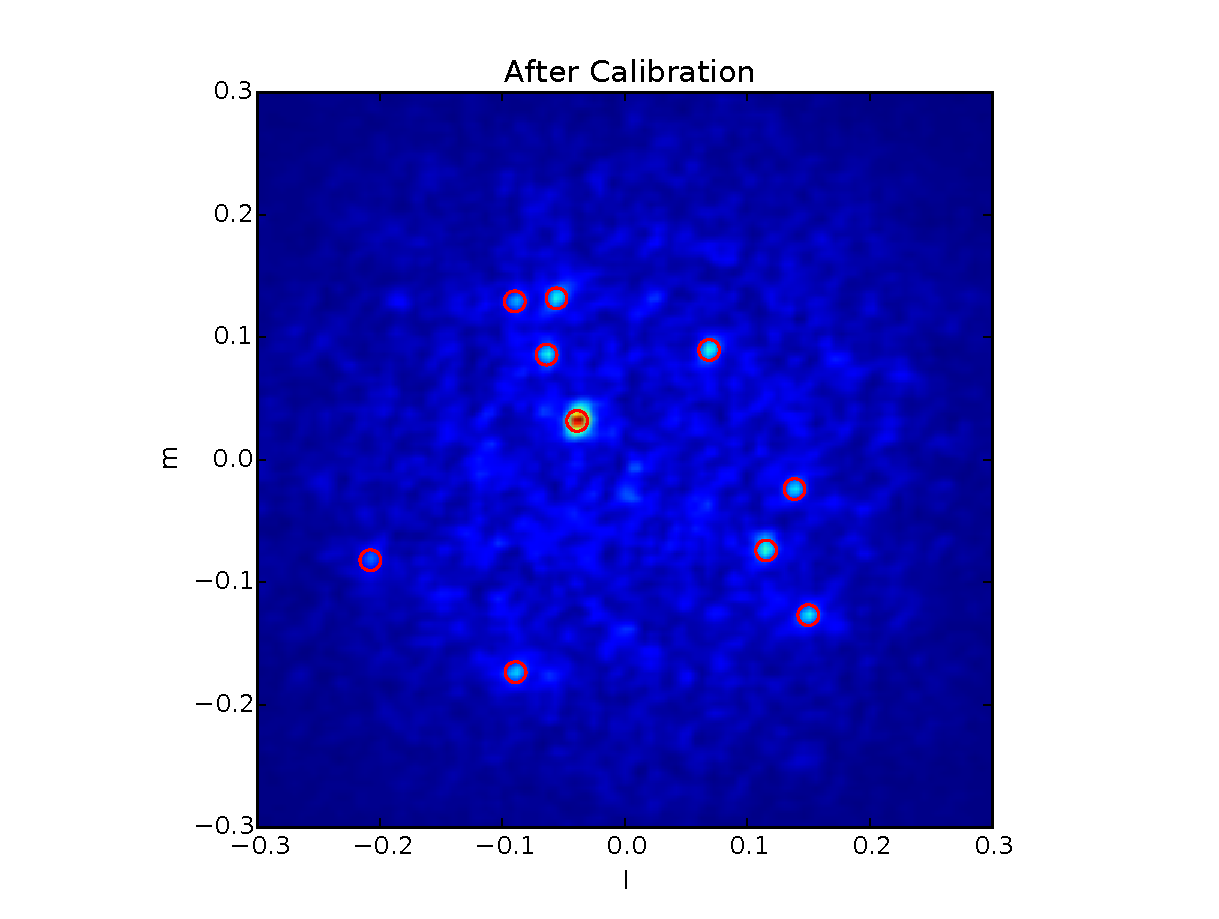
\includegraphics[width=\columnwidth]{figures/cal_paper_sim_image_after.pdf}
\caption{Images formed during simulated calibration. \emph{Top:} An image generated from a single frequency channel and 10 ms integration after the gain estimates are randomized. As expected with random phases, the image is completely noisy, with the shape of the primary beam evident. \emph{Bottom:} An image formed after calibration, again with a single frequency channel and 10 ms integration. The ten simulated (and modeled) point sources are easily visible, and highlighted with red circles.
}
\label{fig:sim_images}
\end{center}
\end{figure}

\section{Application to LWA data}\label{sec:data}
We next demonstrate our calibration algorithm using an observation from the LWA station in New Mexico. The data is from the LWA narrow-band transient buffer (TBN), with time ordered voltage data from 255 antennas within a core radius of 100~m. The central frequency is 74.03 MHz, with a bandwidth of 100 kHz and writeout timescale of 5.12 ms (frequency channel resolution of 195.3125 Hz). For this demonstration we limit ourselves to a single polarization.

After correcting for geometric cable delays, the instrument is naturally well calibrated, as was seen in the demonstration of the EPIC imager in \citealt{thy15c}. However, we will aim to further improve on this calibration using our algorithm.

We proceed by forming model visibilities. We model only two bright objects as point sources: Cyg A with flux 16611.68 Jy \citep{coh07}; and Cas A with flux 17693.9 Jy \citep{kas07}. Because the raw data is attenuated by the primary beam of the instrument, we also account for this in our model using beam values consistent with \cite{hic12}.

We made several choices while studying the behavior of the LWA data to improve our calibration. Through our previous imaging work, we noted that the flux scale of uncalibrated images was consistent with average gain amplitudes of 0.25. To allow the calibration to converge quickly we initialized our gain estimates at this level. We also found a boost in signal to noise is achieved easily by averaging frequency channels and assuming the gains are constant within a sub-band. Here we average solutions across 150 channels, or about 29 kHz. With a fractional bandwidth $B/f_0 = 3.9 \times 10^{-4} \ll 1$, we assume a smooth bandpass across the band. 
A damping factor of $\gamma = 0.7$ was adopted.

Finally, we found that seven antennas\footnote{LWA antenna IDs 48, 85, 124, 148, 203, 217, and 244 were flagged.} produced unstable gain solutions, and in fact corrupted the entire array. We therefore flagged these antennas in our analysis, resulting in a total of 248 antennas to calibrate. In each calibration loop, we form $C_{i,\hat{\boldsymbol{s}}_0}, i=1,2,\ldots N_a$ and update our gain estimates over 10 timestamps (51.2 ms). We iterate the loop 30 times for a total of 1.536 seconds. The results of this calibration experiment are shown in figures~\ref{fig:data_phase}~--~\ref{fig:data_images}.

Figure~\ref{fig:data_phase} shows the phase of our gain estimates over 30 calibration iterations, again with each colored line representing a different antenna. Given the quality of uncalibrated image demonstrated in \cite{thy15c}, it is a bit surprising to see the phase variation in our solutions. However, the phases are relatively flat after about 15 iterations (modulo noise), and exhibit a central ``trunk" where the majority of phases are congregated. This behavior is suggestive that while the uncalibrated voltages were able to produce a viable image, the minor changes from our solutions will focus the image and improve the quality. The actual location of the ``trunk" (slightly negative) is simply determined by the reference antenna chosen to have identically zero phase, but happens to be slightly more positive than the bulk of antennas. For plotting clarity, we unwrapped phases resulting in phases that appear to exceed $\pm \pi$.

\begin{figure}
\begin{center}
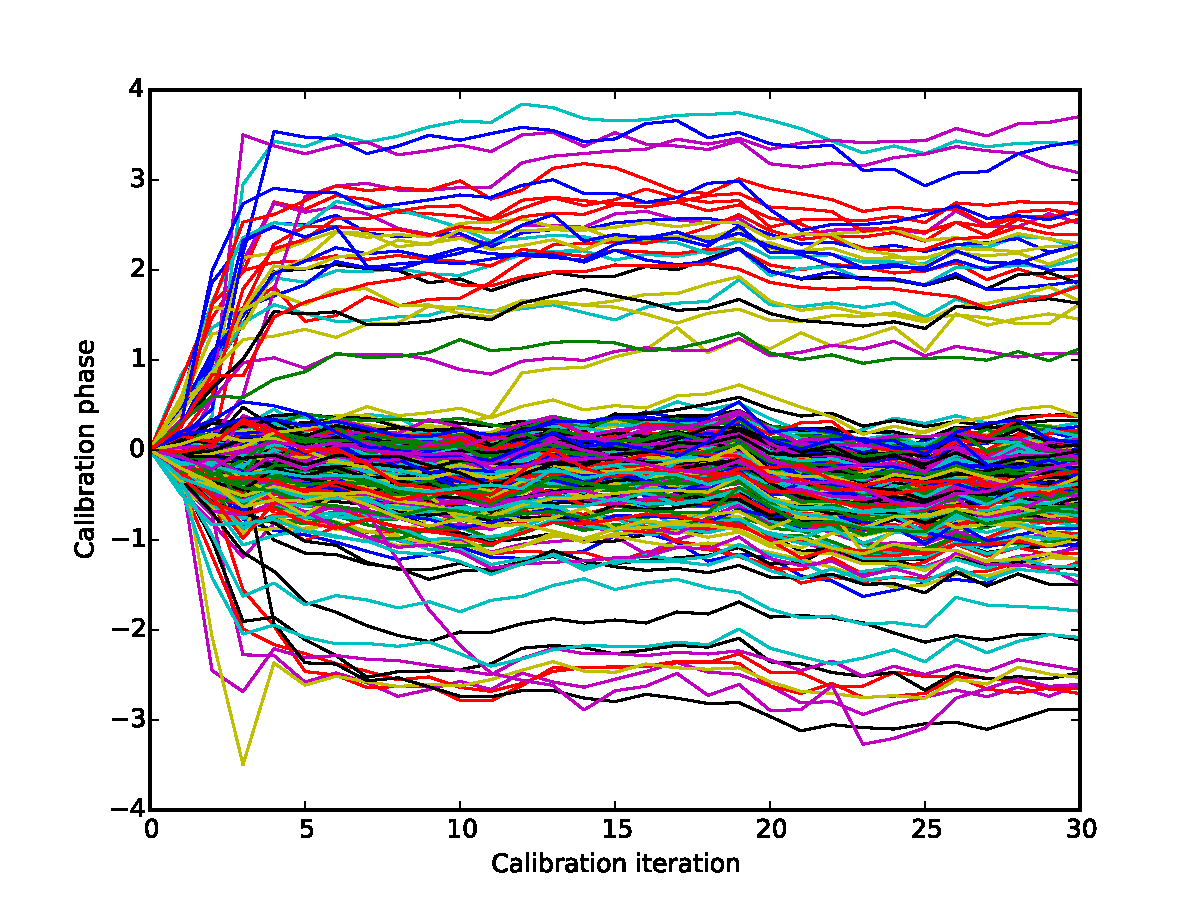
\includegraphics[width=\columnwidth]{figures/cal_paper_data_phases.pdf}
\caption{Gain phase solutions as a function of calibration iteration for an LWA TBN observation. The gain estimates are initialized with zero phase, but quickly span a $2\pi$ range, and settle into relatively flat, albeit noisy, solutions. The majority of phases congregate near zero, which is not surprising given the fairly good quality image produced from uncalibrated data.
}
\label{fig:data_phase}
\end{center}
\end{figure}

The gain amplitudes as a function of calibration iteration are shown in figure~\ref{fig:data_amp}. There is a fairly wide range in gain amplitudes (from 0.12 to 0.59). However, this is not surprising due to the non-uniformity in the cables from the antennas to the receivers. Again, the amplitudes are noisy but relatively flat.

\begin{figure}
\begin{center}
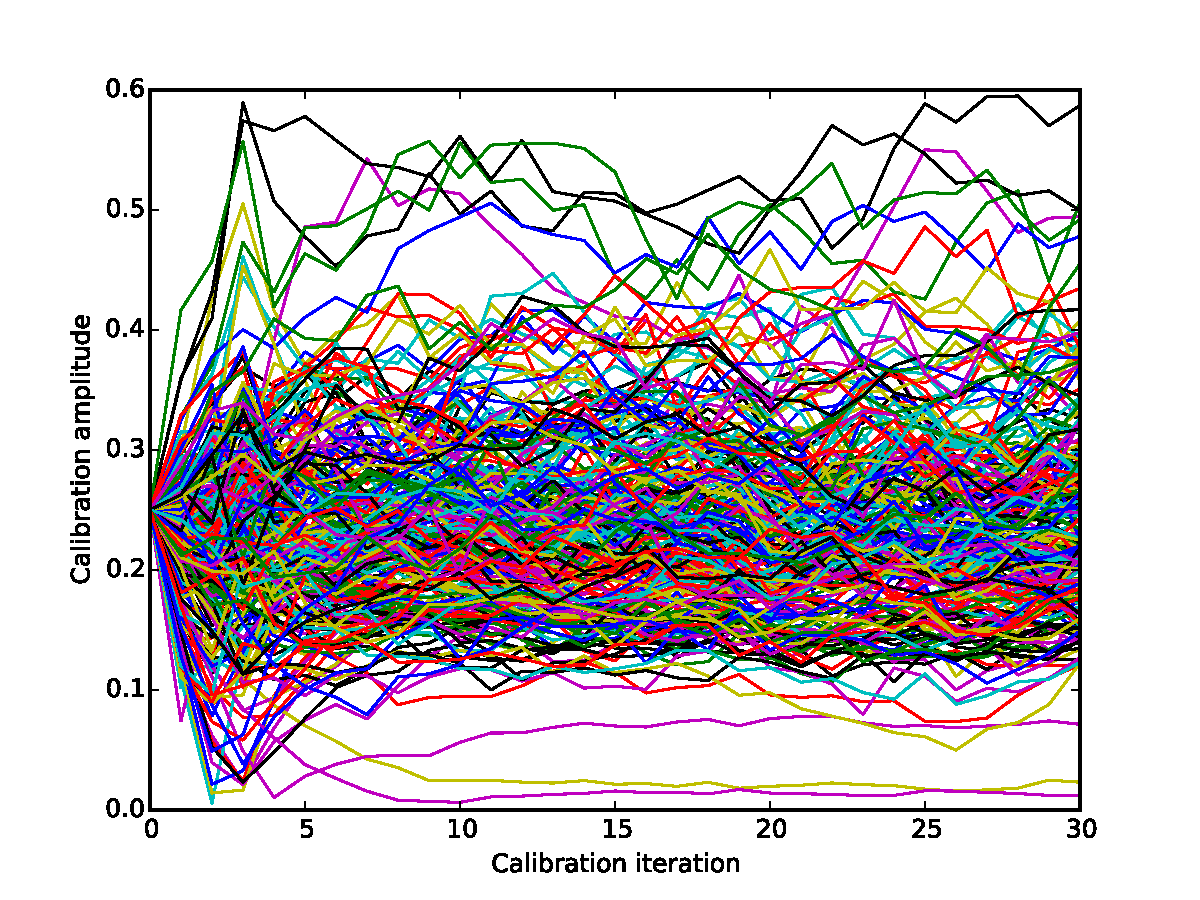
\includegraphics[width=\columnwidth]{figures/cal_paper_data_amps.pdf}
\caption{Gain amplitudes as a function of calibration iteration for an LWA TBN observation. The gains estimates were initialized with amplitude 0.25 after inspection of the electric field values compared to our model sky. The solutions are noisy, but flat. The range in amplitudes is due to the non-uniformity of cables between the LWA antennas and receivers.
}
\label{fig:data_amp}
\end{center}
\end{figure}

Figure~\ref{fig:data_images} shows the improvement in the images due to our calibration. The left panel shows the uncalibrated image integrated over 51.2 ms, 29 kHz. Cyg~A is prominent near the center of the image, and Cas~A is also clearly visible in the upper right. The middle panel shows the image produced after calibration with identical integration time and bandwidth. The sidelobes throughout the image are significantly suppressed, and the galactic plane is much more evident, despite only modeling Cyg~A and Cas~A. We also note that the feature just to the right of Cyg~A is dimmer in the calibrated image, better matching the expected flux from the global sky model (GSM, \citealt{deo08}). We show the GSM\footnote{We use the PyGSM module by D.~C.~Price to import the GSM, https://github.com/telegraphic/PyGSM} modulated by two factors of the LWA power pattern in the right panel of figure~\ref{fig:data_images} for reference.

\begin{figure*}
\begin{center}
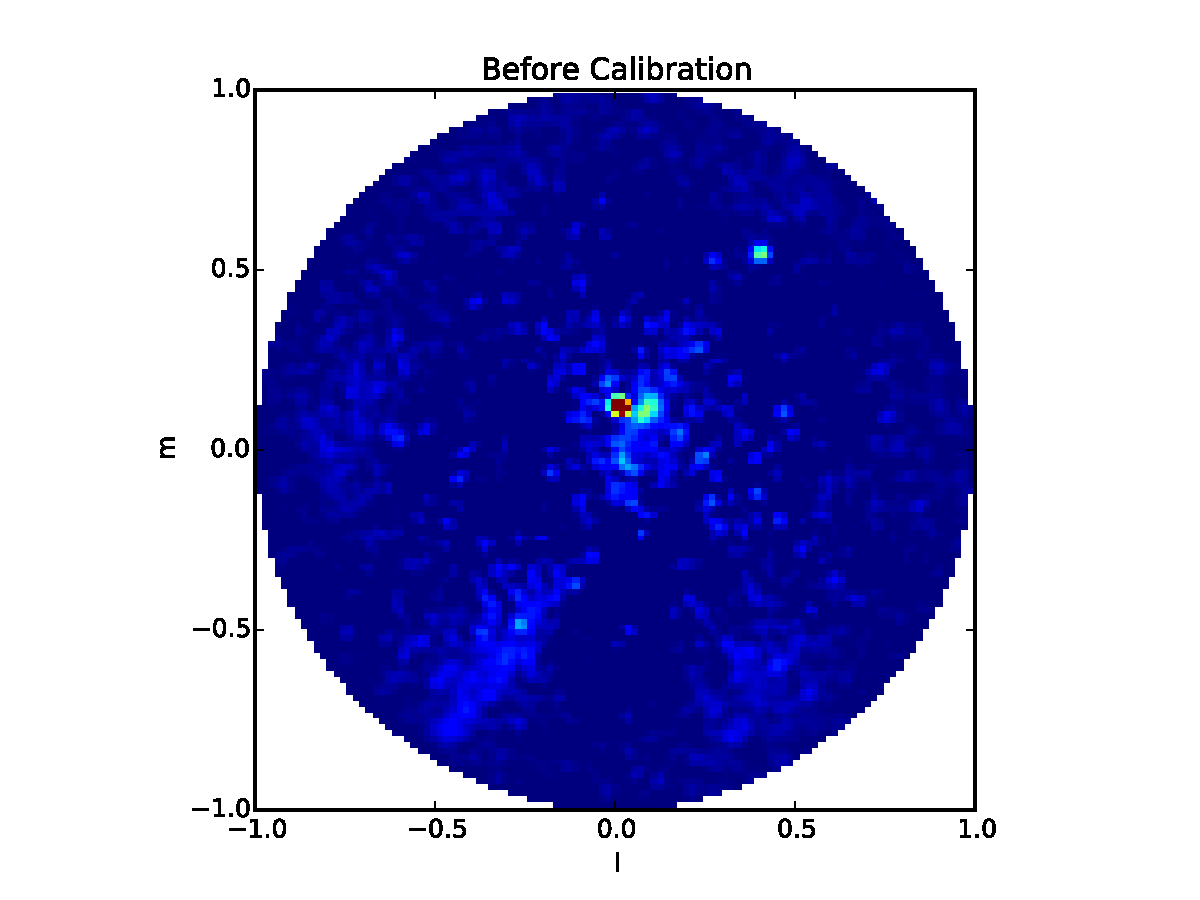
\includegraphics[width=0.33\linewidth]{figures/cal_paper_data_image_before.pdf}
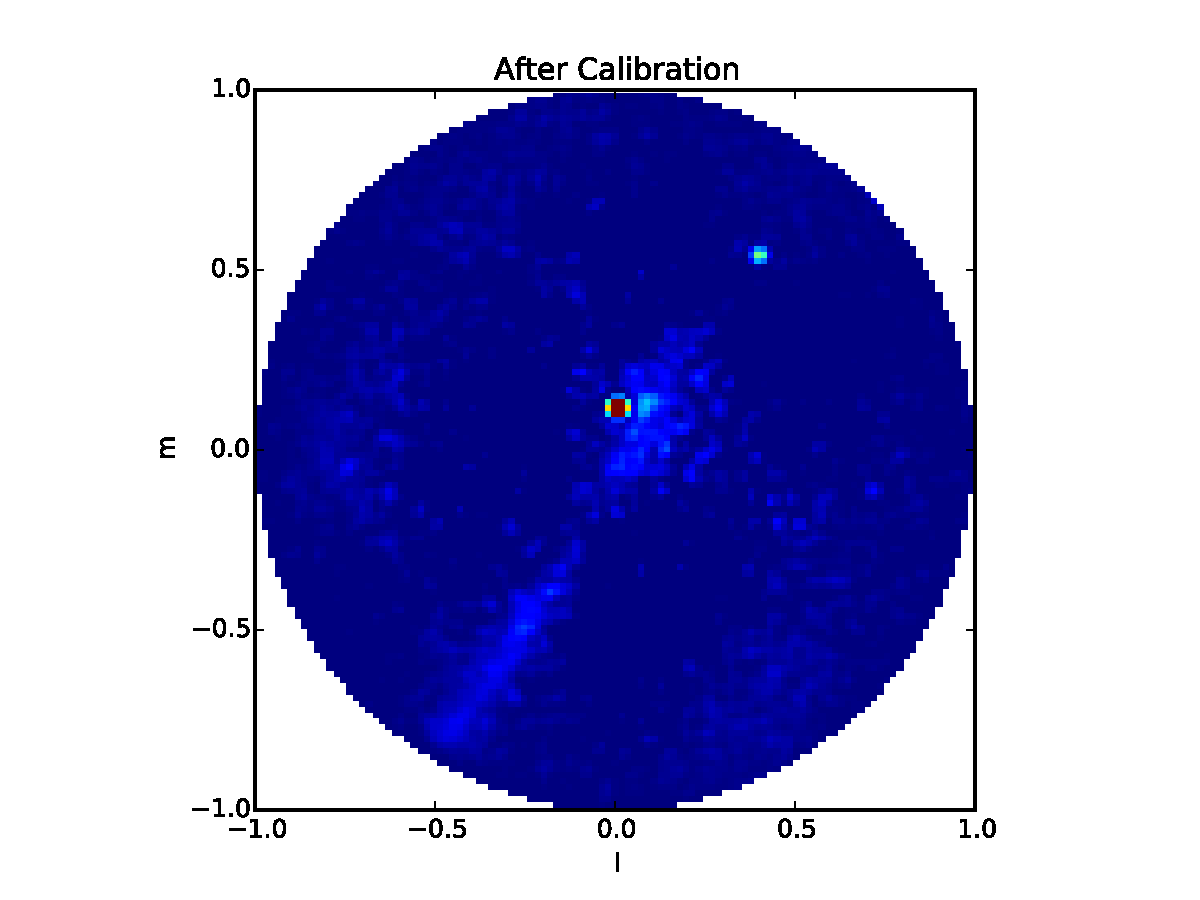
\includegraphics[width=0.33\linewidth]{figures/cal_paper_data_image_after.pdf}
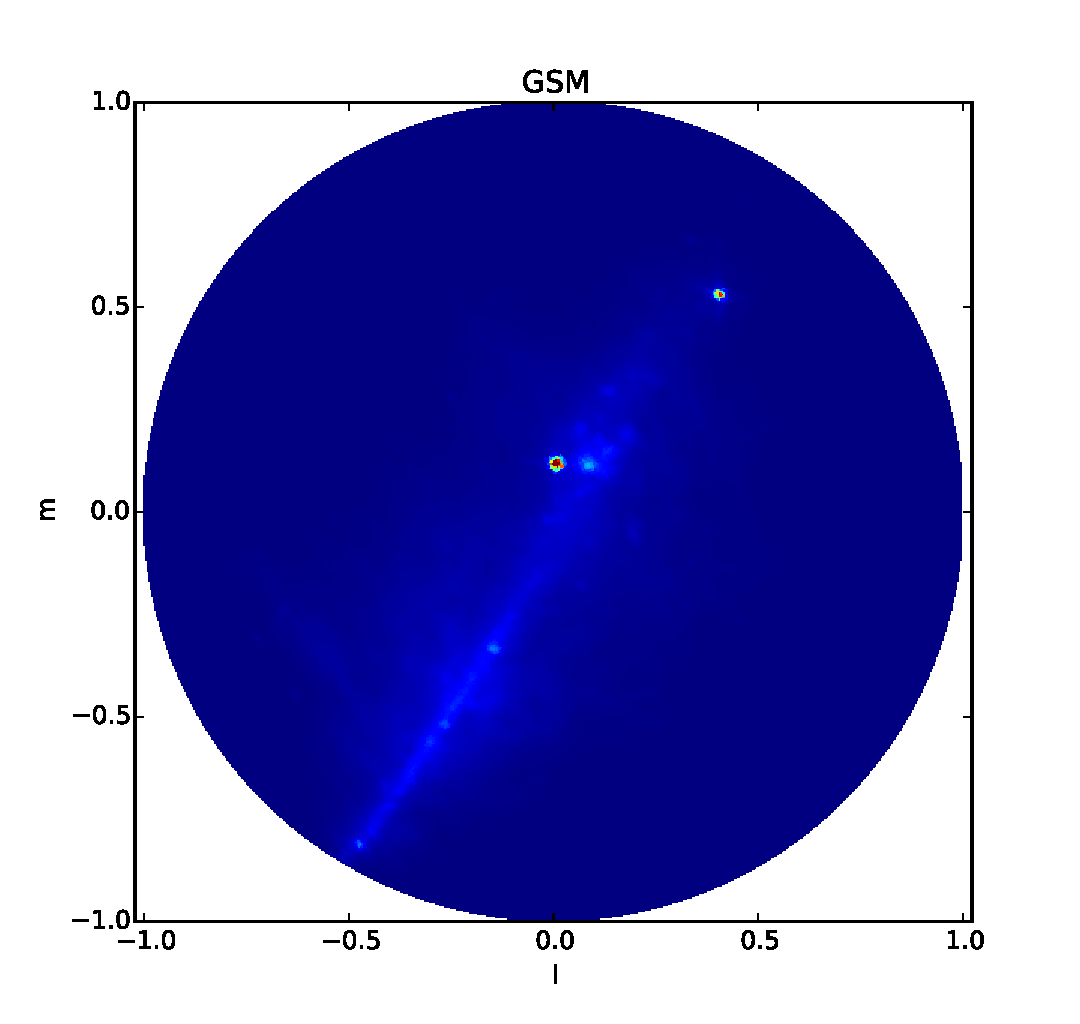
\includegraphics[width=0.33\linewidth]{figures/cal_paper_gsm_beam_weighted.pdf}
\caption{Images produced before (left) and after (middle) calibrating LWA data. These images were produces with 29 kHz bandwidth and 51.2 ms integration. The calibrated image shows significant reduction in sidelobe rumble throughout, while retaining the prominent Cyg~A and Cas~A sources. The galactic plane is also substantially more evident after calibration. For reference, the GSM is shown in the same coordinates and weighted by two factors of the LWA primary beam in the right panel. While much of the GSM is visible in the calibrated image, we note that the model used to calibrate was only the two bright sources, Cyg~A and Cas~A.
}
\label{fig:data_images}
\end{center}
\end{figure*}

To compare the image qualities quantitatively we compute the dynamic range, defined as the peak of the image over the noise level. We estimate the noise level as the median of the absolute deviation of the image, a robust statistic. With this metric we find the calibrated image to have a 55\% dynamic range improvement over the uncalibrated image.

\section{Noise trends and error analysis}\label{sec:noise}
Now we return to simulations to study the effect of noise in our system, and the consequences of an incomplete sky model. We run a suite of simulations varying the receiver noise and integration times, while forming antenna-pixel correlations, $\Cna$, for EPICal gain solutions, and simultaneously forming visibilities from the same E-field streams to find visibility-based gain solutions for comparison. 

We use a simulated sky consisting of a 5~Jy calibrator source, and 49 other random sources with apparent flux densities 0.2 to 0.5 Jy (total sky power $\approx$ 23 Jy). We generated these sources randomly, but kept them fixed for each run. As in section~\ref{sec:sim}, we use the MWA core layout (51 antennas), and a 4.4~m square tophat antenna voltage pattern. We simulate 64 frequency channels each of width 40~kHz. Because our calibration loop treats frequency channels independently, each channel can be treated as a separate trial of the simulation, and is used to better estimate the statistics.

To simulate receiver noise, we add a gaussian distributed complex random number to each antenna electric field measurement at each time stamp according to equation~\ref{eq:apply_gain}. The level of the receiver noise, $\sigma_r = \left<\left|\widetilde{n}_a(f,t)\right|^2\right>$, is varied in different simulation runs. We include two limiting cases, where the receiver noise power is subdominant to the sky power ($\sigma_r = 10.0$~Jy), and where the receiver dominates the noise ($\sigma_r=100.0$~Jy).

For each simulation run we find gain solutions using four methods:
\begin{enumerate}[i.]
\item EPICal, using a full sky model
\item EPICal, using a single point source model
\item Visibility-based, using a full sky model
\item Visibility-based, using a single point source model.
\end{enumerate}
In the cases where we use the full sky model, the model visibilities, $\V'_{ab}$ used in the calibration loop are created using all point sources in the simulated sky. For the single point source model, we only allow the calibration loop to be privy to the bright calibrator source. While we vary the model used for calibration, the simulated ``true sky'' remains fixed with all 50 point sources.

For the EPICal calibration loops, we initialize our gain estimates with the true values (${g^{(0)}_a=g^T_a=1}$), and allow the estimate to be corrupted by the noise through ten iterations of the calibration loop. We adopt a damping factor $\damp=0.35$. Because EPICal updates the gain estimate at each calibration loop, \tcal, but retains a memory of previous iterations through the damping factor, the total integration time is not straightforward. We define an effective integration time by considering the relative weights of each previous $\Cna$ contributing to the current $g^{(n)}_a$ estimate, each with integration time \tcal. In the limit $n\rightarrow \infty$, the geometric series converges to an effective integration time of
\begin{equation}
\teff = \tcal \times \frac{1+\damp}{1-\damp}.
\end{equation}
With the damping factor we adopted here, $\teff \approx 2.1 \times \tcal$. 

We simultaneously form simulated visibilities by correlating all pairs of antenna E-field measurements (including the receiver noise). The E-fields are correlated for a duration equal to the effective integration time of the EPICal loop for comparison. We then find the visibility-based gain estimates by minimizing
\begin{equation}\label{eq:vis_cal}
\chi^2 = \sum_a\sum_{b\ne a} \left|\V_{ab}-g_a g_b^* \V'_{ab}\right|^2,
\end{equation}
using both versions of the model visibilities described above.

 For each version of calibration, we observe the error in the gain estimates averaging over both antennas and frequency channels.
\begin{equation}\label{eq:gain_error}
\sigma_g = \left[\frac{1}{N_f \Nant} \sum_f \sum_a \frac{\left|g'_a(f)-g^T_a(f)\right|^2}{\left|g^T_a(f)\right|^2}\right]^{1/2}
\end{equation}

The results of our simulations are shown in figure~\ref{fig:errors}. The gain errors from our EPICal method is shown with solid lines, while the dashed lines represent the visibility-based calibration. The thick lines represent the results of using a full sky model, and the thin lines are from the single point source model.  In the case of the full sky model, we see the errors trend downward with longer integration times, as expected. The EPICal errors are slightly higher than the visibility-based errors, on average about 23\% difference. This is not surprising as EPICal only uses the information in a single pixel, while the visibilities use all information from the full sky model. However, we see that with this perfect model the errors do behave like noise, and the same level of noise can be achieved with a longer integration time (or larger damping factor).

\begin{figure}
\begin{center}
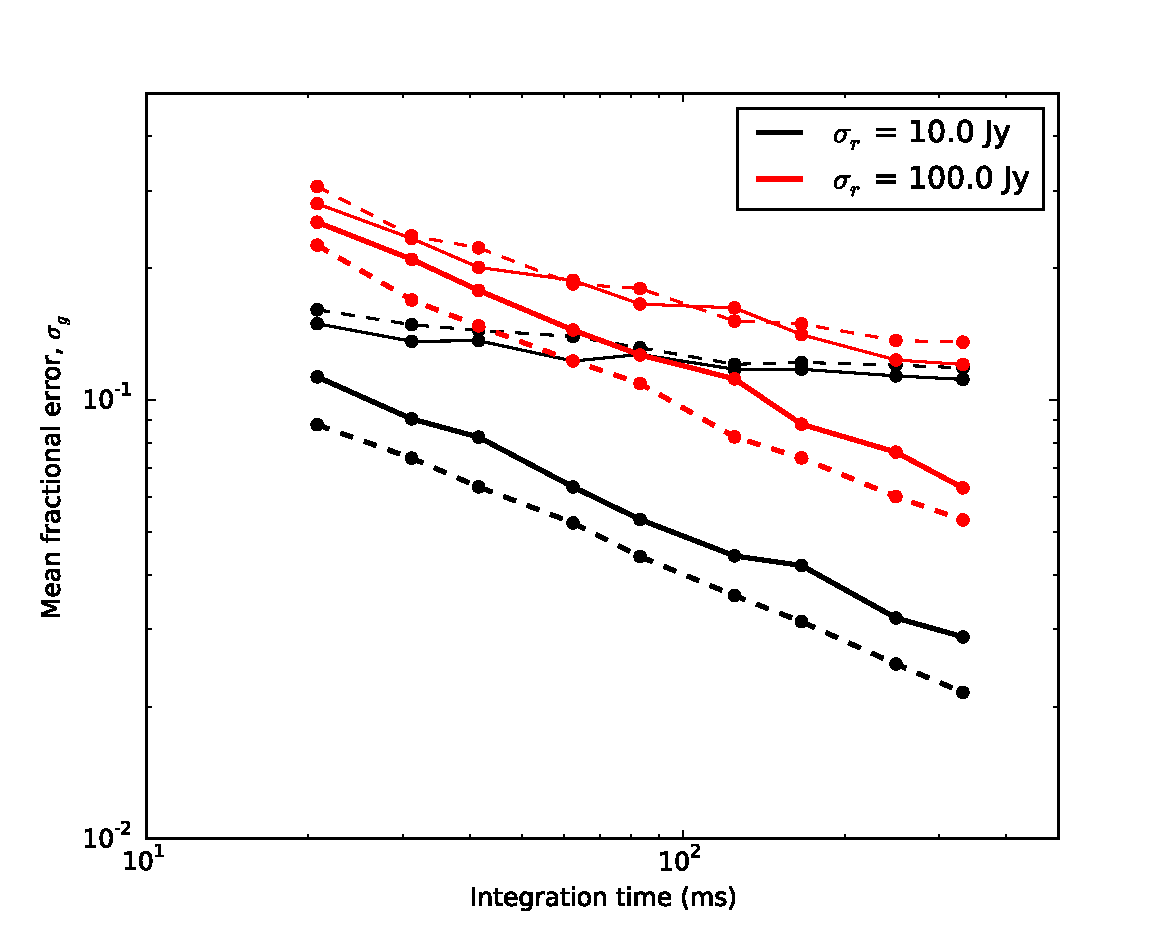
\includegraphics[width=\columnwidth]{figures/cal_paper_errors_complex_sky.pdf}
\caption{Gain estimate errors as a function of integration time, receiver noise (line color), and calibration method. The solid lines represent the error on the EPICal derived gain estimates, while the dashed lines represent the error on the visibility based estimates. The thicker lines were derived using a full sky model in the calibration loops, and the thinner lines used only a single point source model. In the full sky model case we see all methods trend down with longer integration time as expected. For a given integration time, EPICal derived errors are on average 23\% higher than those of visibility based calibration. In the case of a single source model, the errors bottom out due to the flux in the measurements that is not modeled. In this regime the EPICal method performs slightly better than the visibility-based method due to effectively beamforming to the sky pixel where the incomplete model is most accurate. On average EPICal errors are 5\% lower in this regime.
}
\label{fig:errors}
\end{center}
\end{figure}

The exact ratio of EPICal gain noise to visibility-based gain noise depends on the fraction of the total sky power contained in our calibrator source. In the example here, our calibrator accounted for 22\% of the total sky power. We repeated the experiment in the regime where the calibrator dominated the sky and found that the difference in EPICal and visibility-based error goes to zero, as expected. For a typical HERA observation, the sky temperature is expected to by about 180~K \citep{jac15}, and a bright calibrator source could be about 10\% of this power. In this regime we found that EPICal gain noise was about 60\% higher than visibility-based gain noise for the same effective integration time.

When using the single point source model, all calibration methods in figure~\ref{fig:errors} trend downward until they reach an error floor due to the confusion sources that were not modeled. The EPICal and visibility-based solutions reach a similar floor, but EPICal achieves a marginally lower level (on average 5\% lower). This can be attributed to the same reason EPICal underperformed with the full sky model: EPICal only used a single pixel in the sky to form its solutions. When using the full sky model, it was down weighting the information in the rest of the sky. But when the sky model only contains the bright point source, the single pixel used in EPICal is the location where this model is most accurate, effectively down weighting the pixels with incomplete sky model. In the regime typical of HERA discussed above, EPICal's error floor was 10\% lower than that of visibility-based solutions.

Any realistic sky model will lie somewhere between the two extremes explored here. In the case where the sky is modeled by a single source, as is often the case for an initial calibration, EPICal actually achieves smaller gain errors compared to the traditional visibility-based calibration. As the sky model improves, both visibility-based and EPICal gains improve, though the former quicker than the latter. In the limit of a perfect model, both calibration methods produce noise-like errors in their gains which scale down with more integration time.

\section{Discussion}\label{sec:discussion}
Through simulations and application to real data, we have shown that the EPICal algorithm is a viable solution for calibrating direct imaging arrays in real time. The computation necessary only scales with the number of antenna elements, making it a sub-dominant cost factor when designing the correlator. This strategy will enable fast read-out for arrays with many thousands of antennas, which will be necessary for future radio transient and cosmology experiments.

EPICal can be further improved through several extensions. Here we name a few potential considerations for further study. These topics can be thought of as extensions to the white ``estimate gains" box in figure~\ref{fig:schematic}, which can be performed at a much lower cadence than the actual correlations.

\textbf{Multiple pixel correlations.} As was seen in section~\ref{sec:noise}, the single pixel correlation demonstrated in this paper can underperform in the presence of a complex sky, when compared to visibility-based gains with perfect knowledge of the sky. These errors can be mitigated by using correlations of multiple image pixels to incorporate a higher fraction of the total sky power into the calibration loop. Of course this increases the computational cost to a scaling of $\mathcal{O}(\Nant N_{\mathrm{pix}})$, which will typically be much lower than the $\mathcal{O}(\Ng \log_2 \Ng)$ of the correlator itself. These additional correlations would also enable direction dependent gain solutions. Each correlation could be used to independently solve for gains in each pixel direction, then fit to a beam model on the sky. This updated beam pattern would then feed into the gridding step of the correlator, allowing the imager to convolve the signals with the effective beam pattern in the ground plane. 

\textbf{Fitting gain models.} With some knowledge of the instrumental bandpass, the noise of the gain solutions can be greatly reduced by fitting a model to the per-frequency solutions derived here. We used this method at a rudimentary level in our demonstration to LWA data by assuming the gains were constant over a narrow bandwidth. One could easily improve on this by extending the bandwidth and fitting for a low order polynomial in phase and amplitude. Additionally, with knowledge of the poly-phase filters applied to the data stream, we could include channels closer to the edge of the band.

\textbf{Improving sky model.} In this work we used a perfect sky model (for simulation), or a very simple sky model (for LWA data). In principle the images produced by the EPIC correlator can be used to improve the sky model used in calibration -- similar to a major loop in self-calibration. This can be especially useful for compact, widefield arrays which require a model of both compact and diffuse sources over a large patch of sky. In addition to requiring the sky model, the calibration also requires this model to be attenuated by the primary beam, which can be difficult to measure at the precision necessary \citep[e.g.][]{neb15,vir14,thy15b}. However, the direct imaging correlator provides exactly the model necessary in real time, and can be iterated over to improve the images and gain solutions.

\textbf{Dynamic parameters.} In our controlled experiments we fine-tuned a number of parameters based on our testing (e.g. damping factor, integration time, frequency averaging). A deployed system will require robust determination of these parameters to operate continuously. The specifics will be heavily dependent on the stability of the instrument, the frequency of observation, and the sky. For example, a stable instrument may be able to use short integrations to determine a rough estimate of the gains before switching to much longer integration (on order seconds to minutes) to highly increase signal to noise. At low frequencies or high imaging resolution, the dynamics of the ionosphere are important, and will likely drive the limit of time integration allowed.

The work here will serve as a foundation for further development. We have shown that the EPICal algorithm produces reliable calibration solutions, and have identified several aspects to increase the scope. With next generation instruments in the planning and development stages, EPICal is poised to greatly contribute to their success. The software is integrated into the EPIC package and freely available to use in simulations or offline processing of data. Work is underway to port the code to real-time GPU systems for deployment. 

\section*{Acknowledgements}
This work has been supported by the National Science Foundation through award AST-1206552. 
We thank Danny Jacobs for his valuable inputs, and Greg Taylor for providing us with LWA data. 
Construction of the LWA has been supported by the Office of Naval Research under 
Contract N00014-07-C-0147. Support for operations and continuing development of 
the LWA1 is provided by the National Science Foundation under grant AST-1139974 
of the University Radio Observatory program.



%%%%%%%%%%%%%%%%%%%% REFERENCES %%%%%%%%%%%%%%%%%%

% The best way to enter references is to use BibTeX:

\bibliographystyle{../mnras}
\bibliography{../epic} % if your bibtex file is called example.bib


% Don't change these lines
\bsp	% typesetting comment
\label{lastpage}
\end{document}

% End of mnras_template.tex